%%%%%%%%%%%%%%%%%%%%%%%%%%%%%%%%%%%%%%%%%
% FRI Data Science_report LaTeX Template
% Version 1.0 (28/1/2020)
% 
% Jure Demšar (jure.demsar@fri.uni-lj.si)
%
% Based on MicromouseSymp article template by:
% Mathias Legrand (legrand.mathias@gmail.com) 
% With extensive modifications by:
% Antonio Valente (antonio.luis.valente@gmail.com)
%
% License:
% CC BY-NC-SA 3.0 (http://creativecommons.org/licenses/by-nc-sa/3.0/)
%
%%%%%%%%%%%%%%%%%%%%%%%%%%%%%%%%%%%%%%%%%


%----------------------------------------------------------------------------------------
%	PACKAGES AND OTHER DOCUMENT CONFIGURATIONS
%----------------------------------------------------------------------------------------
\documentclass[fleqn,moreauthors,10pt]{ds_report}
\usepackage[english]{babel}
\usepackage{booktabs} % Better Tables
\usepackage{subcaption}
\graphicspath{{fig/}}
\usepackage{svg}




%----------------------------------------------------------------------------------------
%	ARTICLE INFORMATION
%----------------------------------------------------------------------------------------

% Header
\JournalInfo{FRI Natural language processing course 2024}

% Interim or final report
\Archive{Project report} 
%\Archive{Final report} 

% Article title
\PaperTitle{Efficient Fine-Tuning Techniques for Slovene Language Models} 

% Authors (student competitors) and their info
\Authors{Camile Lenderling, Manfred González, and Joaquín Figueira}

% Advisors
\affiliation{\textit{Advisors: Slavko Žitnik}}

% Keywords
\Keywords{LLM, LM, PEFT, NLP, Slovene, LoRA, BitFit, p-tuning}
\newcommand{\keywordname}{Keywords}


%----------------------------------------------------------------------------------------
%	ABSTRACT
%----------------------------------------------------------------------------------------

\Abstract{
This work adapts and evaluates several parameter-efficient finetuning techniques (PEFT) for two large language models: the Slovenian-specific \textit{SloBERTa} and the cross-lingual BERT-Base-Multilingual-Uncased. The study examines methods based on LoRA, bias update, prefix tuning and IA3. Performance is assessed using benchmarks from SloBENCH, a Slovenian language evaluation framework, focusing on the following tasks: natural language understanding, named entity recognition, dependency parsing, and textual entailment recognition. The techniques and models are compared in terms of performance, memory consumption, and runtime.
}

%----------------------------------------------------------------------------------------

\begin{document}

% Makes all text pages the same height
\flushbottom 

% Print the title and abstract box
\maketitle 

% Removes page numbering from the first page
\thispagestyle{empty} 

%----------------------------------------------------------------------------------------
%	ARTICLE CONTENTS
%----------------------------------------------------------------------------------------

\section*{Introduction}

    Large language models and, by extension, language models (LM) in general are becoming ubiquitous in the current technological landscape. As such, the amount of tasks and applications that are being performed by, or with the help of these models is continuously growing. Until recently, LMs were built for specific taks, but with the advent of LLMs this has become both unnecessary, as models are complex enough now that they can perform multiple tasks well out-of-the-box, and unfeasible, as building these models takes an enormous amount of computational resources. However, if one is to achieve the optimal performance on a given task or expand the capabilities of a LM, some adaptations of the model are in order.
    
    These adaptations usually come in the form of a process called fine-tuning, in which the parameters of a pre-trained language model (PLM) are fitted for the specific task we want to achieve. Nonetheless, given the vast number of parameters of parameters in current LLMs, full fine-tuning (FFT) of the weights of a model is usually too computationally prohibitive for most applications. As a result, in the recent years many techniques have been developed to efficiently tune LMs, focusing specifically in reducing the number of trainable parameters (a comprehensive review of this techniques can be found on \cite{survey}). These are usually referred to as parameter efficient fine-tuning techniques (PEFT) and are mainly based on the Lottery Ticket Hypothesis, which states that ``large models are needed in pre-training only to induce (in high probability) the existence of sub-networks initialized with the correct inductive bias for learning.''. In other words, that PLMs already contain the capacity and linguistic ``knowledge'' to perform a wide variety of tasks, but these abilities need to be accentuated through the proper learning stimulus that induces the use of the correct sub-networks when performing a particular task. 

    The purpose of this work is precisely to adapt and evaluate several PEFT techniques with a focus on the Slovenian language. To cover a wide range of approaches the analyzed techniques will span different families: LoRA\cite{hu2022lora} and its derivatives, bias update\cite{bitfit} and soft prompt based techniques. As a base model for analysis the SloBERTa LM will be used, which is a BERT model optimized for Slovenian. For performance assessment the techniques will be evaluated on multiple NLP tasks focused on natural Natural Language Inference (NLI), Name Entity Recognition (NER), Dependency Parsing (DP) and Textual Entailment Recognition (RTE) of the benchmarks provided on the Slobench Slovenian evaluation framework.


%------------------------------------------------
\newpage
\section*{Methods}

\subsection*{LoRA}

The field of adapting large language models (LLMs) for specific tasks has seen significant advancements with the introduction of Low-Rank Adaptation (LoRA). Hu et al.~\cite{hu2022lora} pioneered this approach by freezing the pre-trained model weights and integrating trainable rank decomposition matrices into the Transformer architecture. This method not only substantially reduces the number of trainable parameters required for downstream tasks but also lessens the GPU memory requirements, thereby enabling comparable or superior model quality with notable efficiency. The provision of a package to facilitate the integration of LoRA with PyTorch models, including implementations for popular models like RoBERTa, DeBERTa, and GPT-2, marks a significant contribution to the field.

Further enhancing the parameter efficiency of fine-tuning PLMs, Zhang et al.~\cite{zhang2023increlora} introduced IncreLoRA, an incremental parameter allocation method that judiciously adds trainable parameters based on the importance scores of each module. This approach, distinguished from structured pruning methods, not only improves parameter efficiency but also incorporates early learning and restart warmup techniques to bolster training effectiveness and stability. The method demonstrated superior parameter efficiency and model performance, particularly in low-resource settings, through rigorous experiments on the GLUE benchmark.

On the deployment front, Xu et al.~\cite{xu2023qalora} proposed the Quanti-zation-Aware Low-Rank Adaptation (QA-LoRA) algorithm, aimed at the efficient deployment of LLMs on edge devices. By introducing group-wise operators, QA-LoRA enhances the quantization flexibility while streamlining adaptation, enabling the integration of quantized LLM and auxiliary weights without compromising accuracy. This method stands out by allowing for low-bit inference directly, overcoming the limitations of previous approaches like QLoRA and facilitating faster model deployment on resource-constrained devices.

Lastly, the scalability and efficiency of serving multiple LoRA adapters derived from a base model have been addressed by Sheng et al.~\cite{sheng2023slora} through the introduction of S-LoRA. This system, designed for scalable serving, significantly improves throughput and the capacity to serve numerous task-specific fine-tuned models by employing a unified memory management approach and optimized computation strategies. Complementing these efforts, Gao et al.~\cite{gao2024higher} introduced MoE-LoRA with Layer-wise Expert Allocation (MoLA), which optimizes the allocation of LoRA experts across different layers of the Transformer model, thereby enhancing model efficiency and performance across various NLP tasks. These advancements collectively signify a leap forward in the efficient adaptation, deployment, and serving of LLMs, paving the way for broader application and innovation in the domain.

\subsection*{Bias update}

BitFit\cite{bitfit} is the first recorded technique to have implemented a sparse-finetunning of LMs using only the bias parameters and it falls under the category of partial fine-tuning according to Xu et al.'s taxonomy\cite{survey}. The main mechanism of the technique is simple: during fine-tuning an LM on a particular task update only the bias parameters of the model's encoder layers. These parameters account for only a small fraction of all the parameters of the model (0.1\% in the case of BERT). Additionally, the authors found that fitting only a small subset of these bias parameters (mainly the bias of the query encoders of the attention heads and the biases of one of the layers of the MLP inside of the encoder layer) leads to almost no performance drop and modifies only 0.04\% of the parameters. According to Xu et al. \cite{survey} the technique achieves relatively great results with only a fraction of the memory footprint of other PEFTs. These promising results, combined with the existence of multiple pre-packaged implementations of the technique, led us to choose it as one of the subjects of analysis of this work.  

The findings of the initial BitFit paper were further expanded in the works of Lawton et al.\cite{us-bitfit} using neural architecture search (NAS), more specifically, iterative network pruning. The core idea of the method is to iteratively fine-tune the model using BitFit\footnote{The authors also fine-tuned the models using LoRA, but that falls outside of the scope of this analysis.} and then prune it's bias parameters according to a criteria based on the first order approximation of the loss that results from eliminating certain parameters from the network. The authors found that the resulting network architectures could maintain good performance with a large portion of their bias parameters pruned, further solidifying the findings in the initial BitFit paper that only a relatively small number of bias parameters are responsible for the fine-tuned performance. Unfortunately, there is no code or implementation freely available to replicate the results of this technique in our work.

\subsection* {IA3}

IA3 (Infused Adapter for Attention Approximation) \cite{ia3} is a PEFT technique that focuses on modifying the attention mechanism of a language model by introducing lightweight, learnable adapters that adjust its attention scores. This approach allows for significant reductions in the number of trainable parameters, making fine-tuning more resource-efficient while maintaining or even improving performance on specific downstream tasks. IA3 achieves this by infusing additional parameters only in critical parts of the attention mechanism, thus preserving the core structure and pre-trained knowledge of the original model. The main advantage of IA3 with respect to other PEFT techniques is precisely this infusion mechanism of the learnable parameters, which means that no additional weights have to be added to the model after training and hence inference time remains unchanged.

\subsection*{Soft prompts}
Soft prompts, represent various methods to efficiently adapt LLMs for down-stream tasks without altering the underlying model architecture or weights. This technique involves appending a sequence of tunable tokens, or "soft prompts," to the input of the model. During fine-tuning, these tokens are optimized to guide the model towards generating the desired task-specific output. Two prominent methods for implementing soft prompts are prompt tuning and prefix tuning (P-tunning). 

\subsubsection*{Prompt tuning}
Prompt tuning introduces a set of $\ell$ learnable tokens (soft prompts), denoted as $P =  \{P_1, P_2, \dots P_\ell$\},  and concatenates these tokens to beginning of the input to the model $X \in \mathbb{R}^{n\times d}$ to form $\hat{X} \in \mathbb{R}^{(n + \ell) \times d}$. Throughout the fine-tuning process, only the parameters associated with the prompt tokens $P$ are adjusted via gradient descent, while the pre-trained model parameters are kept fixed. Hence, the length of the prompt and the dimensionality of the token embeddings determine the parameter cost for fine-tuning.~\cite{prompt_tuning} 

\subsubsection*{Prefix-tuning}
Prefix-tuning introduces the idea of appending a set of soft prompts $P =  \{P_1, P_2, \dots P_\ell$\}, not to the input layer but to the hidden states within the multi-head attention layers of the model. This is different from prompt tuning, which concatenates  soft prompts directly to the input. To promote stability during training, a feed-forward network (FFN) is used to parameterize these soft prompts. During fine-tuning, two distinct sets of prefix vectors, $\hat{P}_K$ and $\hat{P_V}$, are concatenated to the attention layer's original key ($K$) and value ($V$) vectors, respectively. Hence, the only parameters that require optimization are those of $\hat{P}_K$, $\hat{P_V}$, and the FFN. Once the model is fine-tuned, the FFN is no longer needed, and only the optimized key and value prefix vectors are kept for model inference.~\cite{prefix_tuning}


\section{Proposed Methodology}
This section outlines the methodology used in our experiments, covering data preparation, model fine-tuning, evaluation, and resource measurement.

\subsection{Data Preperation}
We began by selecting datasets from the SloBench framework, specifically focusing on the tasks of Natural Language Inference (NLI), Named Entity Recognition (NER), Dependency Parsing (DP), and Recognizing Textual Entailment (RTE). The SI-NLI dataset was chosen for NLI, the SSJ500K dataset was used for both NER and DP, and the SuperGlue Human-based RTE dataset was employed for the RTE task. Data preprocessing involved tokenizing the text using appropriate tokenizers for SloBERTa and BERT-Base-Multilingual-Uncased (BBMU) models.

\subsection{Fine-Tuning Techniques}
We implemented four PEFT methods: LoRA (Low-Rank Adaptation), Bias Update (BitFit), IA3 (Infused Adapter for Attention Approximation), and Prefix Tuning. These methods were selected to cover a range of approaches, from modifying attention mechanisms to introducing trainable tokens. Each technique offers a different strategy for reducing the number of trainable parameters, freezing different parts of the language models to gain resource efficiency.

\subsection{Experimental Setup}
All experiments were conducted on a Tesla V100 GPU on the Arnes HPC cluster. Training parameters such as batch size, number of epochs, and learning rates were standardized across all methods to ensure fair comparisons. For each PEFT technique, we fine-tuned the SloBERTa and BBMU models on the selected datasets. Training was performed for a fixed number of epochs. 

\subsection{Evaluation Metrics}
We assessed model performance using standard metrics: precision, recall, and F1-score. These metrics were chosen to provide a comprehensive view of model accuracy and balance between precision and recall. Additionally, memory consumption and runtime during training were recorded for each PEFT method to evaluate the trade-off between performance and resource efficiency.

\section{Results}
This section outlines the benchmarking results for various Slovene and multilingual large language models (LLMs) applied to different NLP tasks, including Sentiment Analysis (SA), Named Entity Recognition (NER), Dependency Parsing (DP), Natural Language Inference (NLI), and Coreference Resolution (CR). We evaluated the performance using popular Parameter-Efficient Fine-Tuning (PEFT) methods to determine their effectiveness across these different langauage processing tasks.

\subsection{Natural Language Inference (NLI)}
NLI involves determining whether a "premise" sentence logically supports, contradicts, or is neutral to a "hypothesis" sentence. Using the SI-NLI dataset, this study uses $5,937$ Slovene sentence pairs from the Slovenian reference corpus ccKres, each manually annotated with labels of "entailment," "\textit{contradiction}," or "\textit{neutral}."

\begin{table}[ht]
\centering
\caption{Performance Comparison on SI-NLI}
\label{tab:nli_results}
\small
\begin{tabular}{@{}llccc@{}}
\toprule
Model & PEFT Method & Accuracy & F1 Score & Time (s)\\ \midrule
SloBERTa & LoRa & 68.5\% & \textbf{68.0}\% & 260.5 \\
SloBERTa & Prefix Tuning & 35.3\% & 28.9\% & 235.1 \\
SloBERTa & IA3 & 54.9\% & 56.4\% & 245.1 \\
SloBERTa & BitFit & 33.8\% &20.3\% & 106.1\\
SloBERTa & Full & 49.5\% & 47.7\% & 323.3 \\
BBMU & LoRa & 51.7\% & 50.8\% & 297.8 \\
BBMU & Prefix Tuning & 43.8\% & 44.0\% & 237.7 \\
BBMU & IA3 & 52.3\% & \textbf{51.6}\% & 247.2 \\
BBMU & BitFit & 32.2\% & 22.8\% & 107.2 \\
BBMU & Full & 51.1\% & 46.6\% & 321.4 \\
\bottomrule
\end{tabular}
\end{table}

The above results indicate that SloBERTa with LoRa achieves the highest accuracy (68.5\%) and F1 score (68.0\%), while BitFit shows the lowest performance for both models, with accuracies of 33.8\% and 32.2\%. IA3 offers a moderate performance, and Full fine-tuning results in varied outcomes. Training times range from $235$ to $323$ seconds, highlighting efficiency differences among methods.

\begin{figure}[ht]
    \centering
    \includesvg[width=.5\textwidth]{fig/memory_vs_f1_score_nli.svg}
    \caption{Memory (MB) vs. F1-score for various models and PEFT methods for the SI-NLI task. }
    \label{fig:memory_vs_f1}
\end{figure}

In Figure \ref{fig:memory_vs_f1} we observe that  the relationship between memory usage and F1-score performance does not strictly follow the expected exponential trend. Typically, one would expect that increasing computational resources (memory) leads to a proportional increase in performance. However, our results show that this is not always the case.

Methods such as LoRa and IA3 for the SloBERTa model demonstrate high F1 scores with relatively lower memory usage compared to other methods. This suggests that these PEFT methods are more efficient, providing better performance without the need for many computational resources. However, BitFit has lower performance despite its lower memory requirements, indicating that not all PEFT methods offer the same benefits. 


\subsection{Name Entity Recognition (NER)}
The objective of NER is to identify specific key elements in the words of a sentence. For instance, an NER model may be able to identify when a text mentions or refers to a person, a particular location, an organization, etc. In this experiment we use the SSJ500K training dataset to benchmark several PEFT techniques in the same LM as in the previous task: the slovene language specific \textit{SloBERTa} and the multilingual \text{Bert-Base-Multilingual-Uncased} (BBMU). The corpus contains about 500.000 manually annotated tokens for token-level classication in the slovene language. Furthermore, it contains several subsets for different tasks; we used the NER subset which contains roughly 9,500 manually annotated sentences using the entities of the CoNLL-2003 shared task. 

\begin{table}[ht]
\centering
\caption{\textbf{Performance Comparison on SSJ500K's NER subset} The table shows the result of training the {\it SloBERTa} and {\it Bert-Based-Multilingual-Uncased} (BBMU) models using different PEFT techniques and Full Fine-Tunning (FFT) as a baseline in the NER subset of the SSJ500k corpus. All results where generated using three training epochs with batches of 16 samples.}
\label{tab:ner_results}
\small
\begin{tabular}{@{}llccc@{}}
\toprule
Model & Method & Precision & F1 score & Training Time (s)\\ \midrule
SloBERTa & LoRA & 85.7\% & 88.2\% & 85.5 \\
SloBERTa & P-Tuning & 80.8\% & 84.0\% & 68.3 \\
SloBERTa & IA3 & 82.3\% & 85.3\% & 40.2 \\
SloBERTa & BitFit & 14.9\% & 16.9\% & 72.5\\
SloBERTa & FFT & 85.8\% & 88.0\% & 107.5 \\
BBMU & LoRA & 80.0\% & 82.3\% & 115.2 \\
BBMU & P-Tunning & 75.1\% & 78.5\% & 89.8 \\
BBMU & IA3 & 65.1\% & 68.5\% & 95.3 \\
BBMU & BitFit & 17.4\% & 18.5\% & 94.2\\
BBMU & FFT & 80.9\% & 82.8\% & 153.2 \\
\bottomrule
\end{tabular}
\end{table}

The results show decent performance of almost all methods with the \textit{SloBERTa} model, with LoRa even surpassing full fine-tuning with the same amount of training epochs and batch size. Furthermore, all methods reduced considerably the training time over full fine tuning. In fact, Prefix Tuning almost halved the training time of FFT for the \textit{SloBERTa} model, achieving a training time of only 63\% of that of FFT. Additionally, of all techniques LoRA performs by far the best. This is expected as LoRa has proven efficacy. Regarding the other methods, it's surprising that such a simple method as Prefix Tuning can outperform IA3 by such a wide margin in one of the models, specially considering IA3 is intended to be an improvement on LoRA. 

Regarding the performance comparison between the two models, it seems \textit{SloBERTa} performs better overall in all experiments. This is to be expected given \textit{SloBERTa} was specifically trained to perform well in slovene. Additionally, it seems that it responds better to PEFT techniques, hinting at the fact that these techniques may not be as efficient when some cross-lingual transfer learning is required, such as the one required to fine-tune the BBMU model.

Finally, we can see a graph of the different models and techniques combinations performance (f1) vs. memory consumption in figure \ref{fig:memory_vs_f1_ner}. We can observe similar results as in the previous NLI task, where the results don't seem to follow the expected logarithmic curve of diminishing returns. Rather, we see a much flatter curve where the same results can be achieved with an extensively reduced memory footprint. The only outlier seems to be BitFit as seen previously, which, while still using limited resources, achieves very poor performance.

\begin{figure}[ht]
    \centering
    \includesvg[width=.5\textwidth]{fig/memory_vs_f1_score_ner.svg}
    \caption{Memory (MB) vs. F1-score for various models and PEFT methods for the NER task. }
    \label{fig:memory_vs_f1_ner}
\end{figure}



\subsection{Dependency Parsing}

Using a different subset from the previous SSJ500k dataset we developed further experiments to evaluate the techniques' performance in Depedency Parsing (DP). In particular, we wanted to predict for each word, the relation to its root. The subset we used contains about 11 400 synthetically annotated sentences with their corresponding dependency tree. Each word has assigned both a relation to its head or root and an index identifying the mentioned root. We used the same experimental setup as in the previous NER task. The results can be seen in table \ref{tab:dependency_parsing-results}.

\begin{table}[ht]
\centering
\caption{\textbf{Performance Comparison on SSJ500K's DP subset} The table shows the result of training the {\it SloBERTa} and BBMU models using different PEFT techniques and Full Fine-Tunning (FFT) as a baseline in the Dependency Parsing task subset of the SSJ500k corpus. All results where generated using three training epochs with batches of 32 samples.}
\label{tab:dependency_parsing-results}
\small
\begin{tabular}{@{}llccc@{}}
\toprule
Model & Method & Precision & F1 Score & Time (s)\\ \midrule
SloBERTa & LoRA & 94.0\% & 94.1\% & 45.6 \\
SloBERTa & Prefix Tuning & 91\% & 90.9\% & 37.2 \\
SloBERTa & IA3 & 91.9\% & 91.9\% & 39.3 \\
SloBERTa & BitFit & 83.7\% & 82.1\% & 77.8 \\
SloBERTa & FFT & 93.1\% & 93.1\% & 56.0 \\
BBMU & LoRA & 90.4\% & 90.4\% & 58.3 \\
BBMU & Prefix Tunning & 85.6\% & 85.3\% & 50.8 \\
BBMU & IA3 & 85.9\% & 85.5\% & 52.8 \\
BBMU & BitFit & 78.3\% & 77.0\% & 113.9 \\
BBMU & FFT & 90.3\% & 90.2\% & 78.7 \\
\bottomrule
\end{tabular}
\end{table}

In this task we observe similar results as in the previous one. LoRA achieves by far the best results in both models, surpassing FFT with significantly lower training times. However, it seems Prefix Tuning never performs better than IA3. The reason for this may be that the task is relatively more complex, requiring the model to discover deeper relationships between the tokens than in NER, so a more complex approach that focuses on enhancing the attention mechanism of the models may be a better strategy to tackle it. Overall, it seems that PEFT techniques perform quite well, specially with the \textit{SloBERTa} model, obtaining similar or even superior results with significantly reduced training times.

Regarding the comparison between the models, similar results are observed as with the NER task: performance is better in the slovene specific \textit{SloBERTa} and the PEFT methods are less effective in the multilingual model. Finally, just as in the previous experiments, we can see a comparison between memory consumption and performance for this task in figure \ref{fig:memory_vs_f1_dp}. We see almost the same trend as before, with higher, but similar, performance and slightly lower memory consumption. The only difference is that BitFit performs much better in this task, indicating that BitFit seems to be very sensitive to its particular application: it may achieve good results with reduced memory usage on some very specific tasks, while completely failing in others. Finally, BitFit has by far the highest run time.

\begin{figure}[ht]
    \centering
    \includesvg[width=.5\textwidth]{fig/memory_vs_f1_score_dp.svg}
    \caption{Memory (MB) vs. F1-score for various models and PEFT methods for the DP task. }
    \label{fig:memory_vs_f1_dp}
\end{figure}

\subsection{Recognizing Textual Entailment (RTE)}
In this section, we analyze how LoRA fine tunning influnces over the F1 Scores over the SuperGlue Human based RTE dataset from SloBench.
\begin{table}[ht]
\centering
\caption{Performance Comparison on RTE. Mean F1 Score and mean training time over 5 different runs with different seeds.}
\label{tab:rte_results_general}
\small
\begin{tabular}{@{}llcc@{}}
\toprule
Model & PEFT Method & F1 Score & Training Time (s) \\ \midrule
SloBERTa & LoRa & 0.3324 & 17.53 \\
SloBERTa & Prefix Tuning & 0.5492 & 17.01 \\
SloBERTa & IA3 & 0.3235 & 87.67 \\
SloBERTa & BitFit & 0.3919 & 97.94 \\
SloBERTa & FFT & 0.3710 & 10.58 \\
BBMU & FFT & 0.3808 & 51.29 \\
BBMU & BitFit & 0.4783 & 81.78 \\
BBMU & IA3 & 0.4692 & 84.36 \\
BBMU & LoRa & 0.6550 & 24.78 \\
BBMU & Prefix Tuning & 0.4060 & 26.90 \\
\bottomrule
\end{tabular}
\end{table}

\begin{figure}[ht]
    \centering
    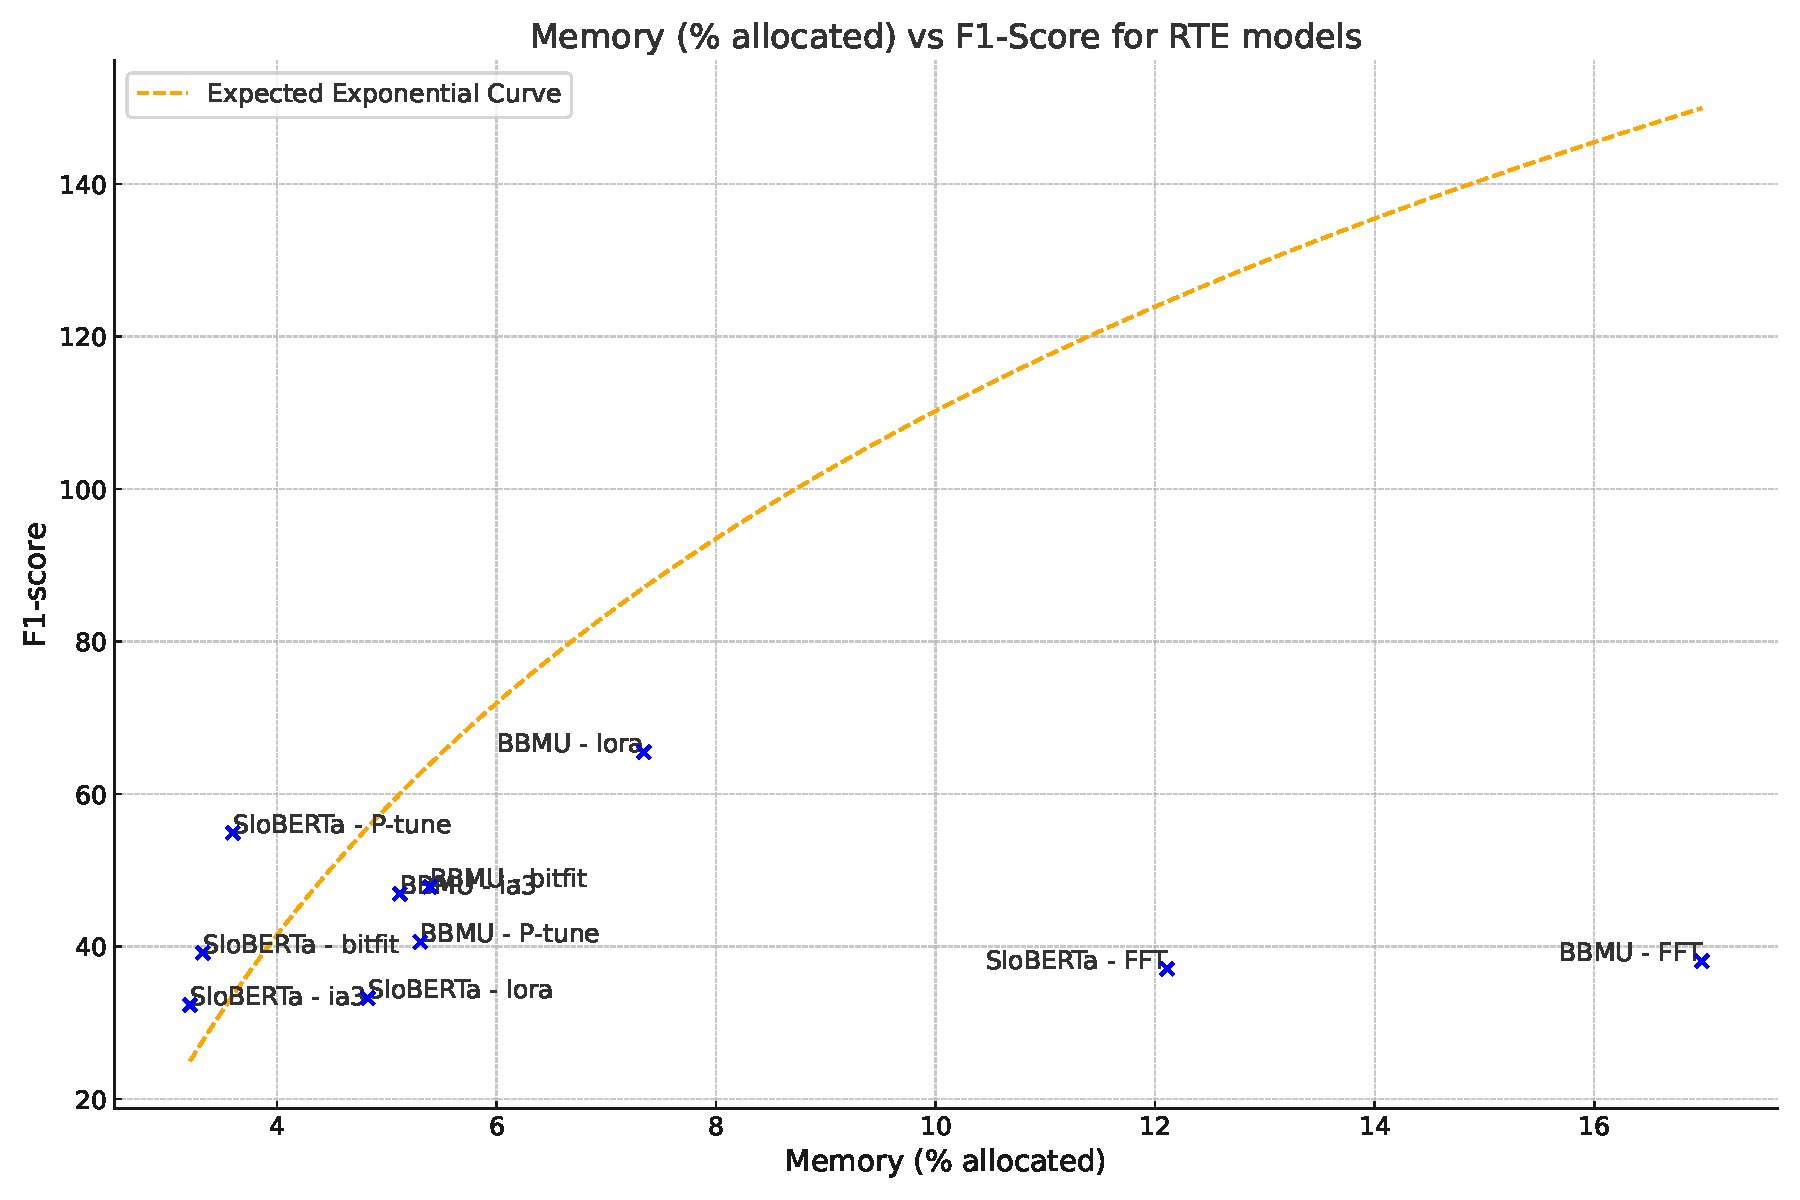
\includegraphics[width=.5\textwidth]{fig/memory_vs_f1_score_rte_models.pdf}
    \caption{Memory (\% allocated) vs. F1-score for various models and PEFT methods for the RTE task.}
    \label{fig:memory_vs_f1_RTE}
\end{figure}


\subsubsection{LoRA hyper-parameter tuning} 
In the table \ref{tab:rte_results_general} we can observe that models like LoRA have bad performance with this small dataset. For this reason we want to explore a bit more this model and see opportunities of improvement by tweaking some of it's hyper parameters. In this experiment, the \textit{SloBERTa} model is fine-tuned on the RTE dataset utilizing the Low-Rank Adaptation (LoRA) approach to explore the impact of various hyperparameters on the model's performance, particularly focusing on the F1 score. The experiment iteratively tests combinations of three key hyperparameters: \( r \), \( \alpha \), and \textit{weight decay}.

\begin{itemize}
    \item \textbf{\( r \) (rank):} This parameter determines the rank of the adaptation in LoRA\cite{hu2022lora}, which affects the model's capacity to learn new patterns without significantly increasing complexity. Values explored were [8, 16, 32], enabling an investigation into how increasing the rank influences learning capacity and generalization.
    \item \textbf{\( \alpha \) (scaling factor):} This controls the scaling of the updates in LoRA\cite{hu2022lora}, impacting how aggressively the model adapts to the new dataset. Tested values were [16, 32, 64], providing insights into finding a balance between overly subtle and overly aggressive updates.
    \item \textbf{Weight Decay (regularization):} Used to prevent overfitting by penalizing larger weights, with values set at [0.01, 0.1, 0.2]. This parameter explores how varying levels of regularization affect overfitting and model performance on validation data.
\end{itemize}

The function used for this experiment orchestrates a grid search over these parameters, training the \textit{SloBERTa} model for each configuration and logging the F1 score to identify the optimal setup. The configuration leading to the highest F1 score is noted as the best, reflecting the most effective balance of learning capacity, adaptability, and regularization for this task. Metrics and configurations are saved, and the best model setup is printed, showcasing the impact of tuning LoRA parameters on model efficacy in a sequence classification task on the RTE dataset. The results can be observed in the figure \ref{fig:lora_params} where the best parameters to be used under this configuration are $r$=16, $\alpha$=64, weight decay=0.1. The best F1 Score achieved with \textit{SloBERTa} was about 0.52 over this dataset, the future work will be focused on compare more models to see which one performs better in this dataset that represents a challenge since it is small and in Slovene.
\begin{figure}[ht!]
\centering

% First subfigure
\begin{subfigure}[b]{0.89\linewidth} % Adjust width to fit the column width
    \centering
    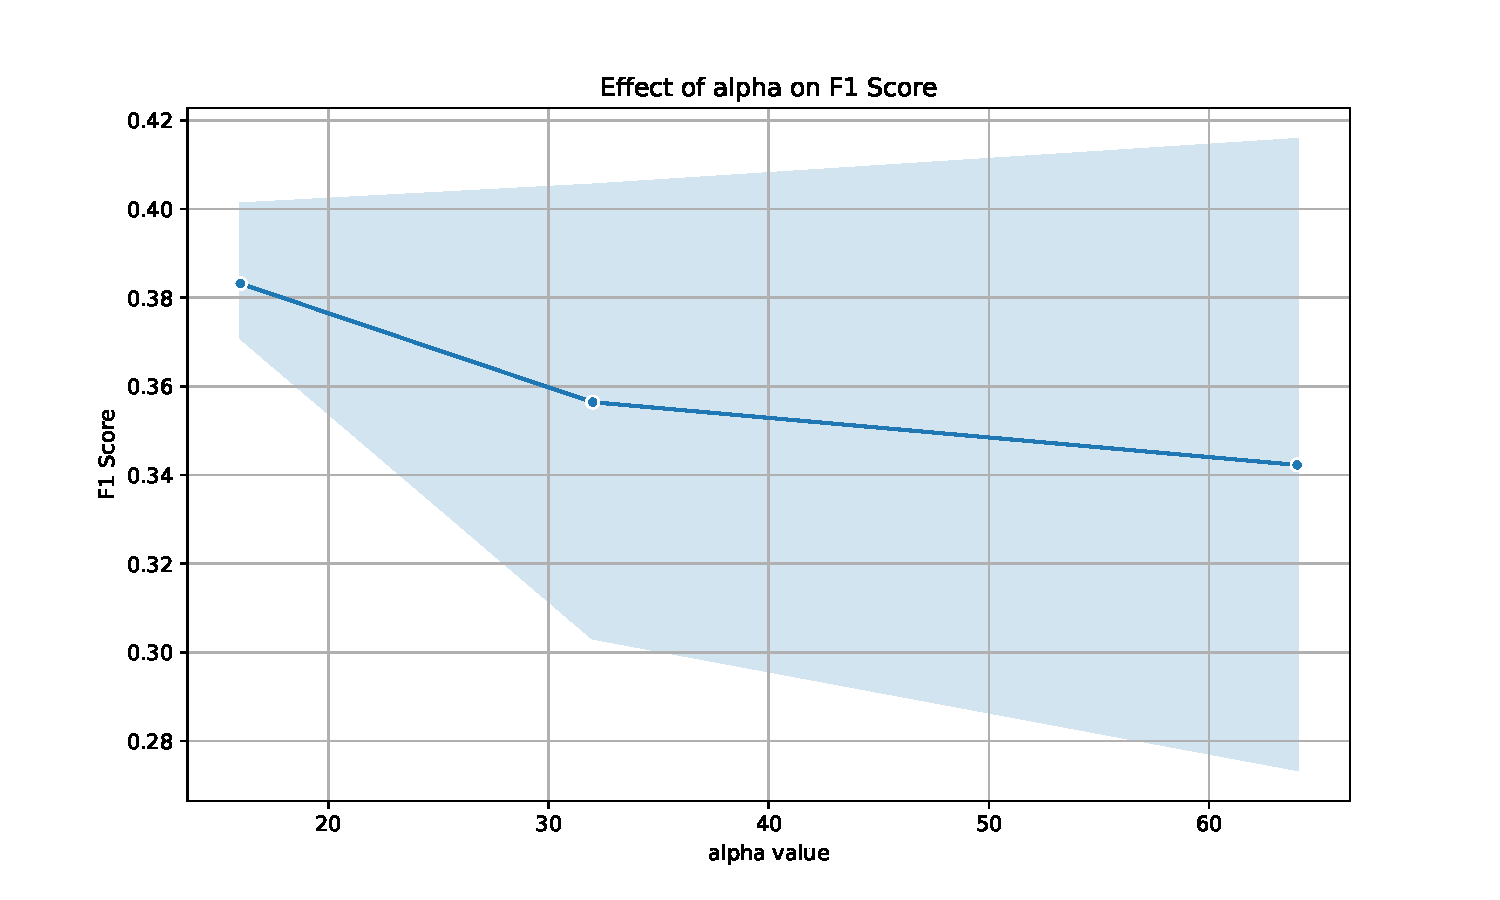
\includegraphics[width=\textwidth]{alpha_on_F1_Score.pdf}
    \caption{Influence of $\alpha$ o in the F1-Score}
    \label{fig:image1}
\end{subfigure}

% Second subfigure
\begin{subfigure}[b]{0.89\linewidth}
    \centering
    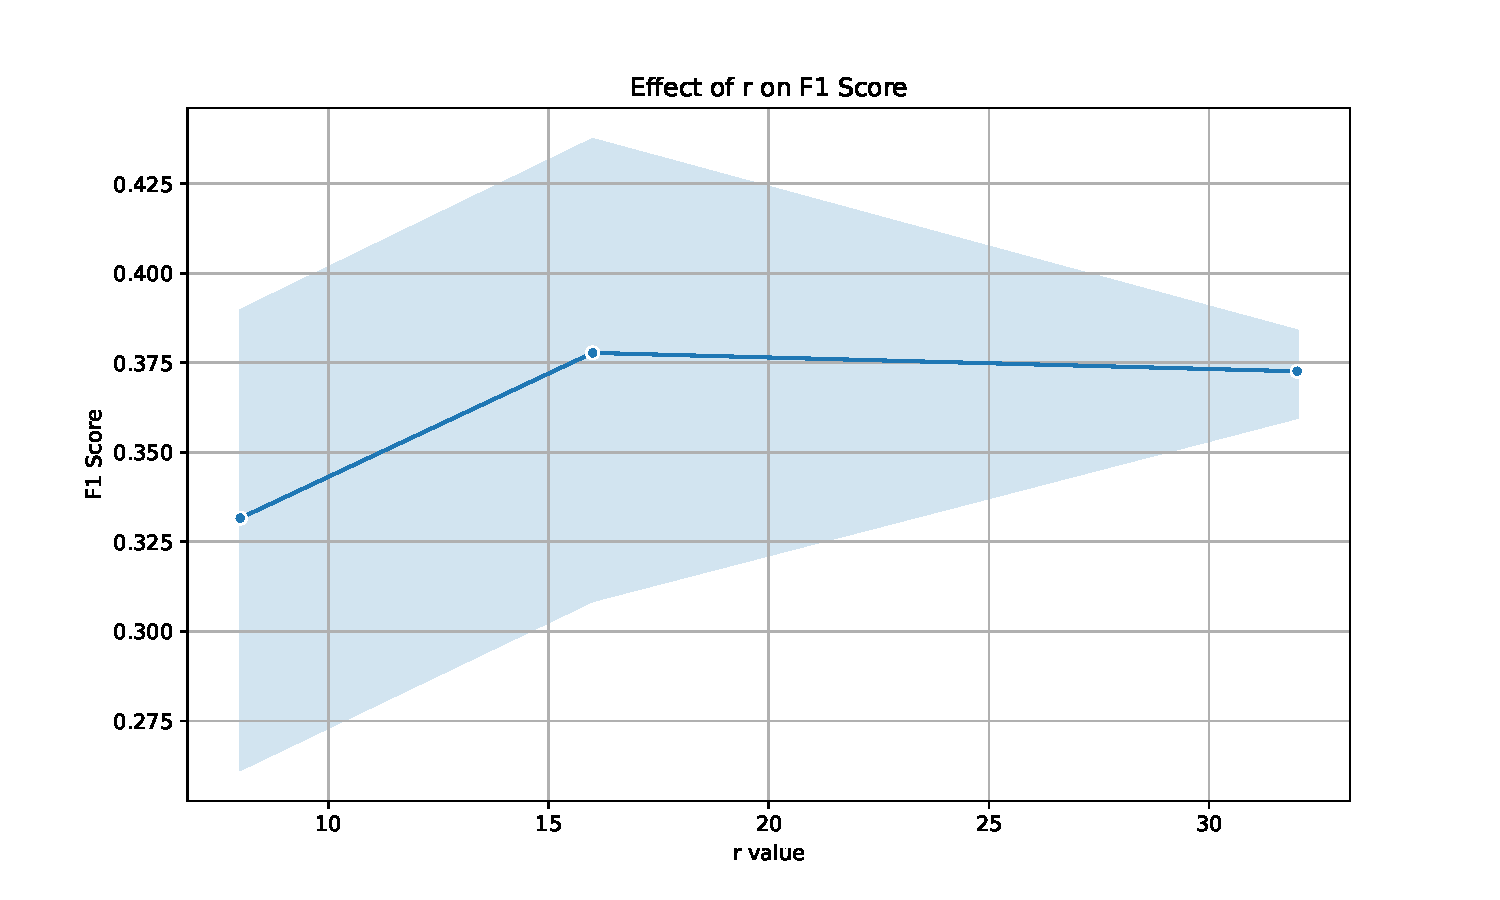
\includegraphics[width=\textwidth]{fig/r_on_F1_Score.pdf}
    \caption{Influence of $r$ or in the F1-Score}
    \label{fig:image2}
\end{subfigure}

% Third subfigure
\begin{subfigure}[b]{0.89\linewidth}
    \centering
    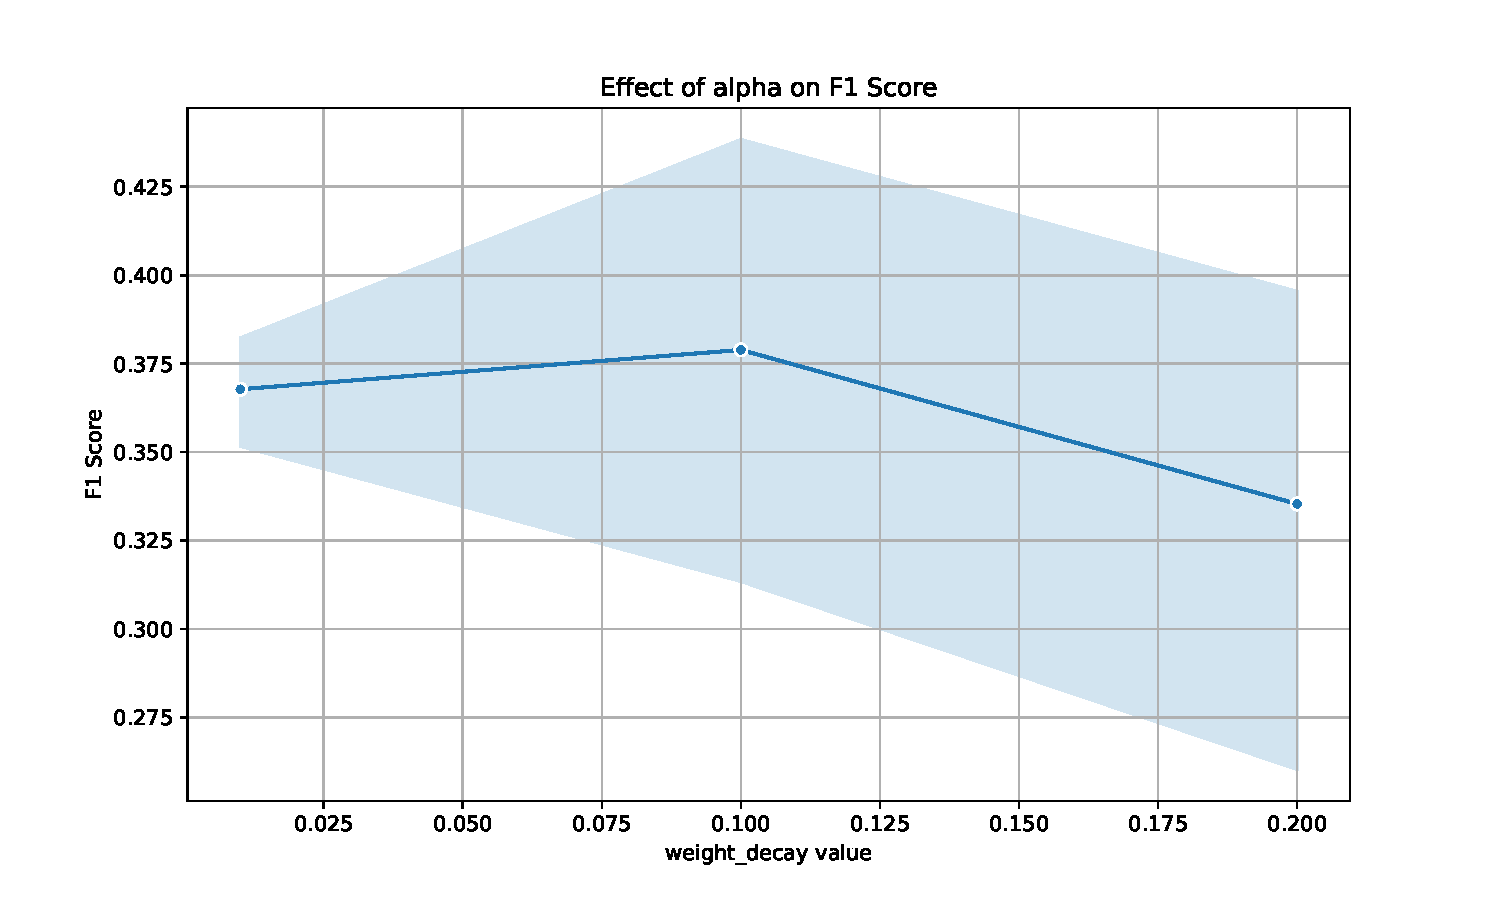
\includegraphics[width=\textwidth]{fig/weight_decay_on_F1_Score.pdf}
    \caption{Influence of weight decay on thein F1-Score}
    \label{fig:image3}
\end{subfigure}

\caption{Different LoRA fine- tunning configurations, results over the F1 Scores using the SuperGlue Human based RTE dataset}
\label{fig:lora_params}
\end{figure}
\subsubsection{RTE best models}
In this subsection we want to explore how early stopping can help by doing the correct parameter setting of these models to achieve better results than \ref{tab:rte_results_general}.
\small
\begin{table}[h]
\centering
\begin{tabular}{@{}llccc@{}}
\toprule
\textbf{Method} & \textbf{Patience} & \textbf{Threshold} & \textbf{Eval F1} & \textbf{Epoch} \\
\midrule
BitFit & 1 & \(1 \times 10^{-3}\) & 0.53 & 15 \\
IA3 & 6 & \(1 \times 10^{-2}\) & \textbf{0.77} & 9 \\
LoRA & 1 & \(1 \times 10^{-2}\) & 0.54 & 3 \\
Prefix Tuning & 3 & \(1 \times 10^{-1}\) & 0.71 & 4 \\
\bottomrule
\end{tabular}
\caption{Best evaluation F1 Scores for each approach with corresponding epoch, patience, and threshold parameters over SloBERTa model.}
\label{tab:best_eval_f1_RTE}
\end{table}
The aim in the experiments of table \ref{tab:best_eval_f1_RTE} was to identify the best combination of patience and threshold values for early stopping that maximizes the F1 score for each fine-tuning approach. We fine-tuned SloBERTa on a specific dataset using four different parameter-efficient methods: LoRA (Low-Rank Adaptation), Prefix Tuning, IA3 (Incremental Adaptation), and BitFit (Bias Fine-Tuning). For each method, we tested a range of patience and threshold values for early stopping. The patience values tested were [1, 3, 5, 6], and the threshold values were [\(1 \times 10^{-1}\), \(1 \times 10^{-2}\), \(1 \times 10^{-3}\), \(1 \times 10^{-4}\)]. Epoch column in the table shows at which epoch the best F1 score was achieved. The patience parameter specifies the number of epochs to wait for an improvement in the validation loss before stopping the training. Threshold parameter defines the minimum change in the monitored quantity to qualify as an improvement. 

The results indicate that different early stopping parameters significantly affect the performance of the fine-tuning methods. Notably, the IA3 method achieved the highest F1 score of 0.77 with a patience of 6 and a threshold of \(1 \times 10^{-2}\). Prefix Tuning also performed well, with an F1 score of 0.71, using a patience of 3 and a threshold of \(1 \times 10^{-1}\). LoRA and BitFit methods showed moderate performance with the best F1 scores of 0.54 and 0.53, respectively. LoRA achieved its best performance with a patience of 1 and a threshold of \(1 \times 10^{-2}\), while BitFit required a patience of 1 and a much lower threshold of \(1 \times 10^{-3}\) to achieve its best result. 

These findings suggest that more aggressive early stopping (lower patience and higher threshold) may not always yield the best performance. Instead, a more balanced approach, with moderate patience and threshold values, appears to be more effective for certain fine-tuning methods. This experiment underscores the importance of tuning early stopping parameters to optimize model performance and convergence. These insights can guide future experiments and practical applications involving the fine-tuning of pre-trained models, especially in resource-constrained environments where parameter efficiency is crucial.

\section*{Discussion}

From the experiments and results we obtained, several conclusions can be drawn. Firstly, LoRA consistently emerged as the best performing method across all tasks, which aligns with its proven efficacy in the literature and its widespread use in the industry. Additionally, both IA3 and Prefix Tuning demonstrated competitive performance with LoRA, offering slightly reduced memory footprints. In contrast, BitFit showed inconsistent performance overall, with memory consumption similar to other methods. In some instances, BitFit's performance was notably poor, occasionally dropping to single-digit F1 scores. This outcome is not surprising, as BitFit represents an early and relatively simplistic approach to PEFT. Although it was pioneering at the time of its development, it has been surpassed by more advanced and sophisticated techniques in the rapidly evolving field of PEFT.

Furthermore, it is important to note that PEFT techniques outperformed full fine-tuning (FFT) on multiple occasions during our benchmarks. This demonstrates that PEFT methods not only make large language models (LLMs) and advanced NLP techniques more accessible to lower-end hardware but also enhance performance on high-end systems. Our results show little to no correlation between memory consumption and performance across all tasks and benchmarks, with minor exceptions due to BitFit's inconsistent performance. 

Given that this work heavily relied on Slovene benchmarks, a few remarks about cross-lingual learning are pertinent. Notably, SloBERTa outperformed BERT-Base-Multilingual-Uncased (BBMU) in all tasks and across all PEFT techniques. This result is expected, as SloBERTa was specifically trained on the Slovene language.  However, the significant performance improvements seen in BBMU when using PEFT methods highlight the effectiveness of these techniques even in cross-lingual settings. 

Finally, we would like to address the sustainability aspect of our work. The widespread use of large language models (LLMs) has a substantial environmental impact~\cite{carbon_footprint} Therefore, adopting PEFT techniques to reduce training time and computational resource requirements represents a significant advancement for the sustainability of the NLP field. The notable reductions in both time and memory usage observed across all models and tasks in our study strongly support this premise. By making NLP more efficient, PEFT techniques not only enhance accessibility but also contribute to more environmentally responsible NLP practices.

%----------------------------------------------------------------------------------------
%	REFERENCE LIST
%----------------------------------------------------------------------------------------
\bibliographystyle{unsrt}
\bibliography{report}


\end{document}